\documentclass[11pt]{amsart}
\usepackage{geometry}                % See geometry.pdf to learn the layout options. There are lots.
\geometry{letterpaper}                   % ... or a4paper or a5paper or ...
%\geometry{landscape}                % Activate for for rotated page geometry
%\usepackage[parfill]{parskip}    % Activate to begin paragraphs with an empty line rather than an indent
\usepackage{booktabs}
\usepackage{graphicx}
\usepackage{amssymb}
\usepackage{epstopdf}
\usepackage{caption}
\usepackage{subcaption}
\usepackage{commath}
\DeclareGraphicsRule{.tif}{png}{.png}{`convert #1 `dirname #1`/`basename #1 .tif`.png}

% Declare commands
\newcommand{\mat}[1]{\mathbf{#1}}
\DeclareMathOperator*{\argmax}{arg\,max}

\title{CS 181 -- Final Project}
\author{Casey Grun, Sam Kim, Rhed Shi}
%\date{}                                           % Activate to display a given date or no date

\begin{document}
\maketitle

% =============================================================================
\section{Overview}

In this project, our challenge was to develop an agent to play a variant of Pac-man, where several aspects of the game's behavior were uncertain. We were tasked with developing an agent that would accumulate as many points as possible by eating ``good'' ghosts, or by eating the ``bad'' ghost after a non-placebo capsule. However, our agent would not know \emph{a priori} which ghosts were good and which was bad, nor would it know which capsules would allow the bad ghost to be eaten (and which were placebos). Finally, Pac-man would lose half a point every turn due to hunger, and would lose a large number of points if caught by the bad ghost without having eaten a capsule.

We therefore had three challenges for this assignment:
\begin{description}
	\item[Capsule clustering] --- 
	\item[Ghost classification] --- 
	\item[Agent development] --- We used reinforcement learning to attempt to train an optimal agent strategy, incorporating information from the ghost and capsule classification data. We also built several agents using hand-coded strategies that incorporated the capsule and ghost classification 
\end{description}

% =============================================================================
\section{Capsule classification}

% =============================================================================
\section{Ghost classification}

% =============================================================================
\section{Agents}

% -----------------------------------------------------------------------------
\subsection{Reinforcement Learning Agents}

In order to explore whether reinforcement learning could be used to train an optimal strategy, we implemented a series of agents that performed reinforcement learning using Q-learning.

Briefly, our agent begins with an estimate of $Q(s,a)$. Upon taking an action $a$ (during epoch $t$), recieving a reward $r$, and observing a transition from $s$
to $s'$, the agent updates our running estimate of $Q(s,a)$ as follows:
$$Q(s,a) \gets Q(s,a) + \alpha_k(s,a) \left[ (r + \gamma \max_{a' \in \mathcal{A}} Q(s', a')) - Q(s,a) \right].$$

We got best results when the learning rate $\alpha$ was set to 0.01 for the first 1000 epochs, after which it was set to 0.001. The optimal value for the discount factor $\gamma$ was about 0.4; these were determined by coordinate descent. 

A key challenge was determining how the many-dimensional, partially-observable game state could be discretized into a single, discrete state representation $s$. We therefore experimented with several ``basis functions'' for representing the state space. We built three different agents that utilized different basis function representations:

\begin{description}
	\item[GhostPositionAgent] --- $s = ((p_x, p_y), (g_x, g_y), (b_x, b_y), (c_x, c_y), h)$ where $(p_x, p_y)$ is the position of Pac-man, $(g_x, g_y)$ is the position of the good ghost $(b_x, b_y)$ is the position of the bad ghost, $(c_x, c_y)$, is the position of the nearest non-placebo capsule, and $h$ is 1 if Pac-man has eaten a capsule (e.g. the bad ghost is currently scared). The positions $(p_x, p_y), (g_x, g_y), (b_x, b_y), (c_x, c_y)$ were each binned into $n$ bins, such that there were $n^{2 * 4} * 2$ possible states. This agent attempts to learn a direction to move for each configuration.
	\item[LocalNeighborhoodAgent] --- $s = ((g_x, g_y), (b_x, b_y), (c_x, c_y), h)$. Similar to GhostPositionAgent; however, positions are stored relative to Pac-man himself. Each dimension is binned into one of $n$ values; if one of the objects is a distance of more than $r$ away from Pac-man in one dimension, it is classified in the most distant bin in that dimension. This agent attempts to reduce the effective dimensionality of the GhostPositionAgent, but maintains the directional information lost by the GoodBadCapsuleDistanceAgent. This agent attempts to learn a direction to move for each configuration.
	\item[GoodBadCapsuleDistanceAgent] --- $s = (g, b, c, h)$ where $g$ is the distance to the nearest good ghost, $b$ is the distance to the bad ghost, $c$ is the distance to the nearest non-placebo capsule, and $h$ is 1 if Pac-man has eaten a capsule (e.g. the bad ghost is currently scared). Each of the distances $g$, $b$, and $c$ were sorted into one of $n$ bins, where $n = 5$, such that the size of the state space was $n^3 * 2$. Unlike the other two agents, this agent attempts to learn \emph{which object to pursue} (the good ghost, the bad ghost, or the capsule). Once the learner has selected the object to pursue, the agent will move in whichever legal direction minimizes the distance to the target.  
\end{description}

In an attempt to improve the rate of convergence, recognizing in particular that Q-learning is much slower to propagate negative rewards than positive rewards, we implemented two learners that were ``seeded'' with initial values for the rewards for various actions:

\begin{description}
	\item[SeededGoodBadCapsuleDistanceAgent] --- Same as GoodBadCapsuleDistanceAgent; however, chasing the bad ghost without the capsule was assigned $Q = -1200$, regardless of the distance.
	\item[SeededLocalNeighborhoodAgent] --- Same as LocalNeighborhoodAgent; however, any action which moved towards the bad ghost without the capsule was assigned $Q = -1200$ if the bad ghost was within the radius $r$ of Pac-man.
\end{description}

% -----------------------------------------------------------------------------
\subsection{Hand-coded Agents}


% -----------------------------------------------------------------------------
\subsection{Agent comparison}

\begin{figure}
	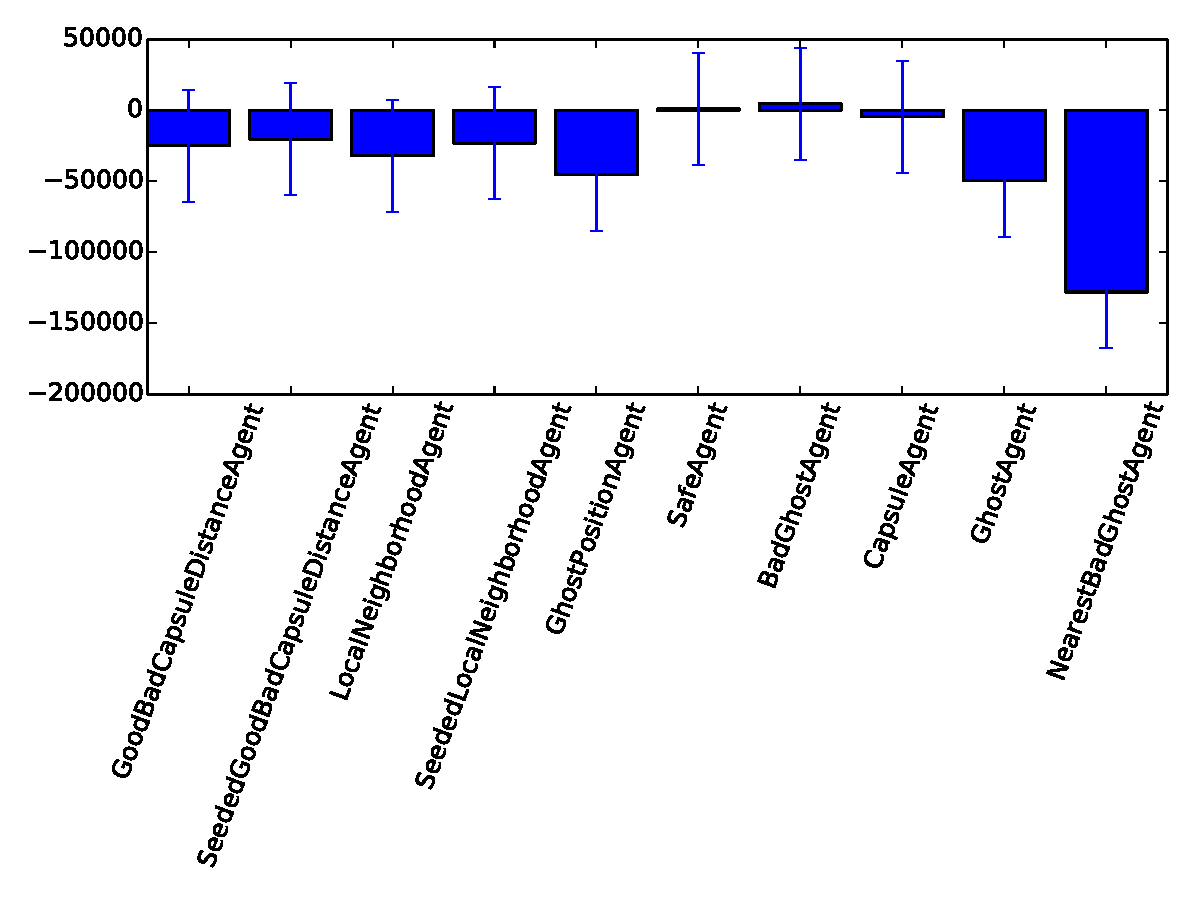
\includegraphics[width=\textwidth]{agents-finals.pdf}
	\caption{Final scores (after 1000 game steps) for each agent (mean $\pm$ std. dev., $n = 10$ games for each agent)}
\end{figure}

\begin{figure}
	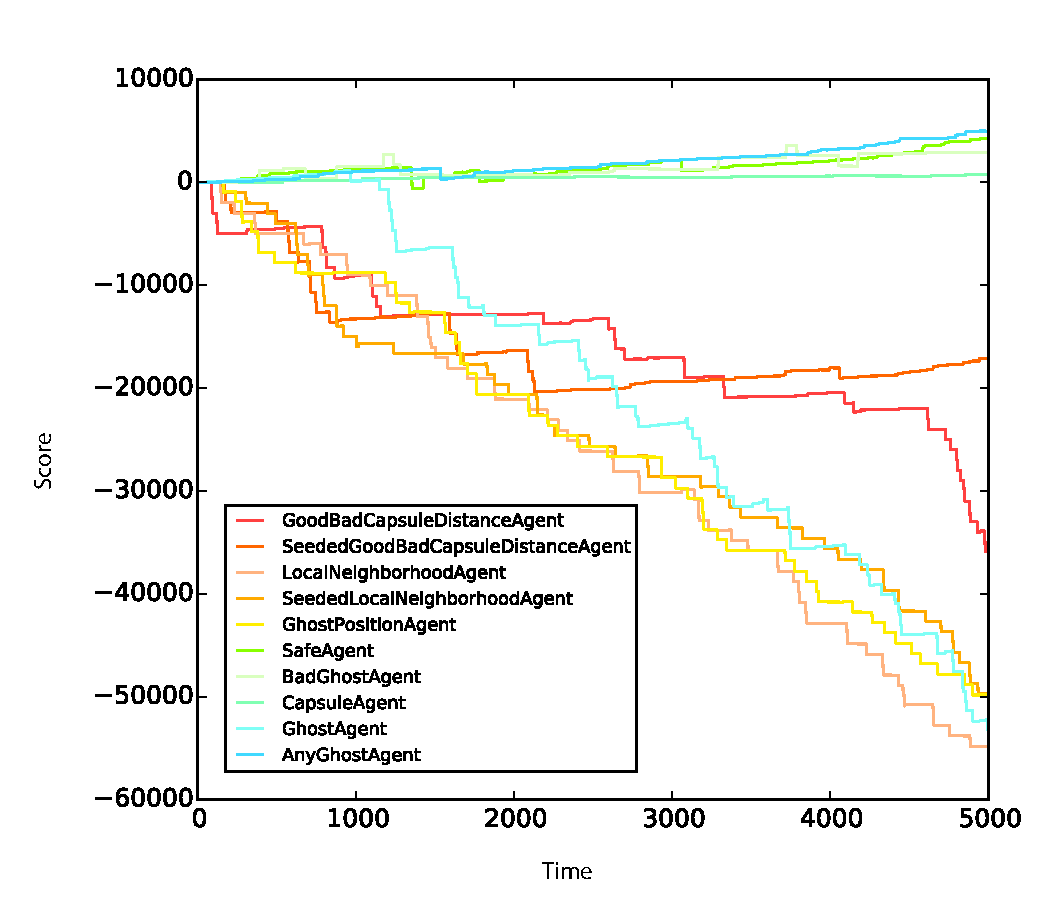
\includegraphics[width=\textwidth]{agents-trajectories.pdf}
	\caption{Representative trajectories of each agents: game step vs. score.}
\end{figure}


% =============================================================================
\section{Conclusion}


\end{document}